\documentclass[a4paper,12pt]{jarticle}
\usepackage{comment}
\usepackage[top=20truemm,bottom=20truemm,left=20truemm,right=20truemm]{geometry}
\usepackage[dvipdfmx]{graphicx}
\usepackage{here}
\usepackage[utf8]{inputenc}
\title{情報と産業・社会 レポート1 課題2}
\author{学生番号\\氏名}
\date{平成29年6月27日}
\begin{document}
\maketitle
\tableofcontents
\section{はじめに(目的)}
%文章で4~5行程度にまとめる。
%「課題」についての背景、経緯、目的などを述べる。
%「まとめ(結論)」と対応させる。
課題:\\
「ビッグデータと人工知能が産業構造を変える」ことの内実について述べよ。\\
以下のことについて調べることを目的とする。
\begin{itemize}
 \item ビッグデータや人工知能がどんなものなのか知る。
 \item ビッグデータや人工知能が将来産業構造に与える影響を知る。
 \item より一般的に、ITの発達によって社会全体がどのように変化するかを考察する。
\end{itemize}
%なぜそのように変わるのかも述べる。
\newpage
\section{調査方法}
%具体的な調査方法を箇条書き、または図(絵)を使ってわかりやすく説明する。
%2ページ以内でまとめる。
インターネットを使用して調査した。
\begin{center}

\includegraphics[width=100truemm]{computer_search_kensaku.png}
\end{center}
\section{調査結果}
%調査結果を箇条書き、または図(グラフ)を使ってわかりやすく説明する。
%2~3ページ程度にまとめる。
\begin{description}
 \item[調査対象]\mbox\\\\
 \item[ビッグデータとは?]\mbox\\\\
 ビッグデータは典型的なデータベースソフトウェアが把握し、蓄積し、適用し、分析できる能力を超えたサーズのデータで、多量性(事象を構成する個々の要素に分解し、把握・対応することを可能とするデータ)、多種性(各種センサーからのデータ等、非構造なものも含む多種多様なデータ)、リアルタイム性(リアルタイムデータ等、取得・生成頻度の時間的な解像度が高いデータ)という3つの特徴が挙げられる。ITの発達により、このような特徴を持ったデータを扱えるようになり、異変の察知や近未来の予測等を通じ、利用者個々のニーズに即したサービスの提供、業務運営の効率化や新産業の創出等が可能となる。
  \begin{figure}[H]
   \begin{center}
    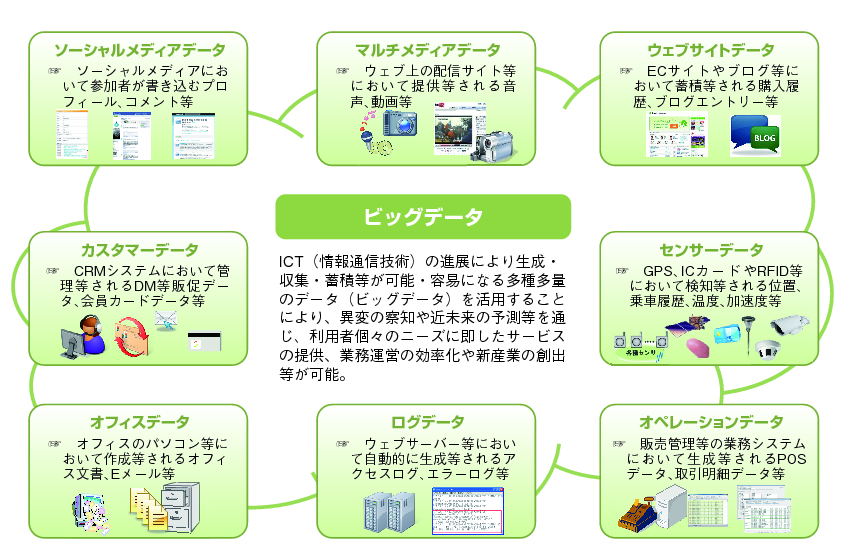
\includegraphics[width=150truemm]{BigData.png}
    \caption{様々なビッグデータ}
    \label{BigDataPicture}
   \end{center}
  \end{figure}
 \item[人工知能とは?]\mbox\\\\
 人工知能開発には、「人間の知能そのものを持つ機械を作る」と、「人間が知能を使ってすることを機械にさせる」という2つの立場があり、現在の人工知能の研究のほとんどは後者の立場をとっている。遺伝と淘汰を用いてプログラムを生成する遺伝アルゴリズムや、専門家の知見をルールとして蓄積し,推論の手法を用いて問題を解決するエキスパートシステムなど、人工知能研究の中には様々な分野が存在する。
  \begin{figure}[H]
   \begin{center}
    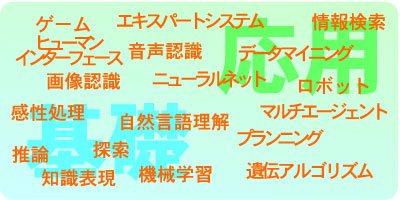
\includegraphics[width=150truemm]{AI.jpg}
    \caption{人工知能の様々な研究分野}
    \label{AIPicture}
   \end{center}
  \end{figure}
\newpage
 \item[産業構造への影響]\mbox\\\\
 今回は日本における産業構造への影響に絞って調査した。
 \begin{itemize}
  \item 日本の産業の衰退\\
 半導体、液晶テレビ、携帯電話など、過去に強い競争力を誇った日本の産業はその競争力を失い、製品が市場に広がるスピードが加速している中、日本の産業がそのシェアを失うスピードも加速しているというのが現在の日本の産業の現状であり、ビッグデータ、人工知能がこれからどのように産業構造に影響を与えるかを見極めて、その変化に柔軟かつ迅速に対応することで競争力を回復させることが目指されている。
  \item 「モノ」から「システム」への価値の移行
 これまで、「モノ」は人間がある目的のために操作していたが、人工知能が発達することによって機械自体が目的を理解し、もはや操作することなく目的が達成されるようになる。そうなったとき、「モノ」の利用者にとっての価値は「モノ」単体の使いやすさから、モノ(ハードウェア)、ソフトウェア、データを含むシステム全体の価値へと移行する。\\
例えば、
   \begin{itemize}
    \item 自動車の運転という人間の行為が、ビッグデータ・人工知能によってシステムが代替できるようになれば、車両(ハードウェア)単体では、独立した価値評価の対象ではなくなり、「快適・安全・安価な移動」を実現してくれるシステム全体が価値評価の対象となる。
    \item 自らの快適な室温に「調節」という人間の行為を、AI・ビッグデータによってシステムが代替できるようになれば、「エアコン」や「サーモスタット」単体は、独立した価値評価の対象ではなくなり、「快適空間」を実現してくれるシステムが、全体として価値評価の対象となる。
   \end{itemize}
ということが起こりうる。
  \item 産業活動のプロセスのシステム化
   ビッグデータ、人工知能の発達によって産業活動のプロセス(生産スケジューリングや設備の保全管理等の工場 オペレーション、品質保証・メンテナンス、マーケティング、在庫管理)は、需要 予測、設備の稼働状況、部品の劣化状況、顧客の嗜好の変化等を分析・判 断し、それに基づいて実行されるようになる。また、そのようなシステム化されたプロセスを工場などに提供する企業・ビジネスモデルが登場する可能性がある。\\
例えば、
   \begin{itemize}
    \item 従来は人が行っていた工場の操作が、システムに置き換えられる。そのシステムは工場内で閉じたものではなく、店舗での売上などのビッグデータから需要を予測し、学習していく。
    \item マーケティングにおける発注、出荷、在庫管理がシステム化され、企業の枠を超えて利用される中でさらに学習し、性能を向上させていく。
   \end{itemize}
ということが起こりうる。
 \end{itemize}
\end{description}
\newpage
\section{考察}
%自分がどう考えたか(意見)を根拠(理由)とともに述べる。
%箇条書きで記載する。
\begin{itemize}
 \item ビッグデータと人工知能による知能活動の自動化について\\
 現在発達が進んでいるビッグデータと人工知能の応用によって、これまで人が行ってきた知能的な活動がシステムによって置き換えることができることがわかった。この半世紀でITは急激に発達し、多くのことが自動化されたが、今までに自動化されたことのほとんどは単純作業など、知能を必要としないものだった。コンピュータがビッグデータを扱えるほどの性能と学習能力を得ることで、人間の知能活動さえ自動化されることがわかった。これからもあらゆることが自動化され、「人間にしか出来ないこと」は減り続けていくだろうと考えた。また、あらゆる職業が、それを実現するソフトウェアの開発に置き換えられるだろうと考えた。
\end{itemize}
\section{まとめ(結論)}
%文章で箇条書きに記載する。
%「はじめに(目的)」と対応させる。
\begin{description}
 \item[ビッグデータや人工知能がどんなものなのか知る。]\mbox\\\\
 ビッグデータや人工知能について調査し、それがどんなものなのか、そのように注目されているのかを知った。
 \item[ビッグデータや人工知能が将来産業構造に与える影響を知る。]\mbox\\\\
 ビッグデータや人工知能が日本の産業においてどのような形で注目されているのかを知り、具体的にどんなことがシステム化されると予想されているのかを知った。
 \item[より一般的に、ITの発達によって社会全体がどのように変化するかを考察する。]\mbox\\\\
 調査結果から、ITの発達によって社会全体が受ける影響を考察することが出来た。 
\end{description}
\section{参考文献}
%題目、著者名、雑誌(書籍)名、年号、ページを必ず記載する。
\begin{thebibliography}{99}
 \bibitem{BigData} 総務省 ビッグデータとは何か\\
http://www.soumu.go.jp/johotsusintokei/whitepaper/ja/h24/html/nc121410.html
 \bibitem{AI1} 人工知能学会 人工知能って何?\\
https://www.ai-gakkai.or.jp/whatsai/AIwhats.html
 \bibitem{AI2} 人工知能学会 人工知能研究\\
https://www.ai-gakkai.or.jp/whatsai/AIresearch.html
 \bibitem{IndustrialChange} ビッグデータ・人工知能がもたらす経済社会の変革\\
http://www.meti.go.jp/committee/kenkyukai/sansei/kaseguchikara/pdf/010\_03\_03.pdf
\end{thebibliography}
\end{document}
